% Compiles with pdfLaTeX (Overleaf default), XeLaTeX or LuaLaTeX
\documentclass[aspectratio=169]{beamer}
\usepackage[T1]{fontenc}
\usepackage[utf8]{inputenc}
\usepackage{tgheros}\renewcommand{\sfdefault}{qhv}
\newcommand{\head}{\fontseries{b}\selectfont}
\usepackage{newunicodechar}
\newunicodechar{≤}{\ensuremath{\le}}
\newunicodechar{≥}{\ensuremath{\ge}}
\newunicodechar{≈}{\ensuremath{\approx}}
\newunicodechar{÷}{\ensuremath{\div}}
\newunicodechar{−}{\ensuremath{-}}
\newunicodechar{²}{\textsuperscript{2}}
\newunicodechar{³}{\textsuperscript{3}}
\newunicodechar{⁴}{\textsuperscript{4}}
\usepackage{tikz}
\usepackage[most]{tcolorbox}
\usepackage{array,booktabs,colortbl}
\graphicspath{{figs/}}

% ---------------- colours ----------------
\definecolor{ink}{HTML}{14213D}
\definecolor{paper}{HTML}{F7F5F0}
\definecolor{paperb}{HTML}{ECE8DF}
\definecolor{soft}{HTML}{4A5568}
\definecolor{orng}{HTML}{D9662B}
\definecolor{lorng}{HTML}{F0A46F}
\definecolor{blu}{HTML}{2F6FB0}
\definecolor{line}{HTML}{CFC8BA}
\definecolor{cardbg}{HTML}{FFFDF8}
\definecolor{pillo}{HTML}{F3D2B9}
\definecolor{pillb}{HTML}{CFE0F2}
\definecolor{darktext}{HTML}{C9CFDA}
\definecolor{lighttext}{HTML}{F2EFE8}

\setbeamertemplate{navigation symbols}{}
\setbeamersize{text margin left=1.07cm,text margin right=1.07cm}
\setbeamercolor{normal text}{fg=soft}
\setbeamercolor{background canvas}{bg=paper}
\setbeamertemplate{itemize item}{\color{soft}\textbullet}

% ---------------- type scale (1920 px = 16 cm) ----------------
\newcommand{\eyebrow}[1]{{\fontsize{6.2}{8}\selectfont\bfseries\color{orng}#1\par}\vspace{1.6mm}}
\newcommand{\ttl}[1]{{\head\fontsize{15}{17}\selectfont\color{ink}#1\par}\vspace{3.2mm}}
\newcommand{\lead}[1]{{\fontsize{9.5}{12.8}\selectfont\color{ink}#1\par}}
\newcommand{\body}[1]{{\fontsize{7.6}{11}\selectfont\color{soft}#1\par}}
\newcommand{\smalltxt}[1]{{\fontsize{6.2}{8.6}\selectfont\color{soft}#1\par}}
\newcommand{\foot}[1]{\begin{tikzpicture}[remember picture,overlay]\node[anchor=south west,text width=13.9cm,inner sep=0] at ([xshift=1.07cm,yshift=0.53cm]current page.south west){\fontsize{5.7}{7}\selectfont\color{soft}#1};\end{tikzpicture}}
\newcommand{\hl}[1]{{\color{lorng}#1}}

% cards, pills, callouts
\newtcolorbox{card}[1][]{enhanced,colback=cardbg,colframe=line,boxrule=0.4pt,arc=1.7mm,left=3mm,right=3mm,top=2.6mm,bottom=2.6mm,#1}
\newtcolorbox{callout}[1][]{enhanced,colback=ink,colframe=ink,arc=1.7mm,left=3.5mm,right=3.5mm,top=2.6mm,bottom=2.6mm,fontupper=\fontsize{8}{11}\selectfont\color{lighttext},#1}
\newcommand{\pill}[2][pillo]{\tikz[baseline=(p.base)]\node[fill=#1,rounded corners=1.6mm,inner xsep=1.8mm,inner ysep=0.7mm](p){\fontsize{5.7}{7}\selectfont\bfseries\color{ink}#2};\par\vspace{1.2mm}}
\newcommand{\cttl}[1]{{\fontsize{7.6}{10}\selectfont\bfseries\color{ink}#1\par}\vspace{1mm}}
\newcommand{\clbl}[1]{{\fontsize{6.6}{9}\selectfont\color{soft}#1\par}}
\newcommand{\cnum}[2][orng]{{\head\fontsize{17}{18}\selectfont\color{#1}#2\par}\vspace{1.2mm}}

\newcommand{\darkslide}{\setbeamercolor{background canvas}{bg=ink}}
\newcommand{\altslide}{\setbeamercolor{background canvas}{bg=paperb}}
\newcommand{\plainbg}{\setbeamercolor{background canvas}{bg=paper}}

% tables
\newcommand{\tsz}{\fontsize{6.6}{9}\selectfont\color{ink}}
\newenvironment{dtable}[1]{\tsz\renewcommand{\arraystretch}{1.35}\begin{tabular}{#1}\arrayrulecolor{line}}{\end{tabular}}

\begin{document}

%================ 1 cover
{\darkslide
\begin{frame}[c]\relax
\eyebrow{\color{lorng}MAJOR PROJECT · DEPARTMENT OF COMPUTER SCIENCE AND ENGINEERING, NITK SURATHKAL}
{\head\fontsize{22.5}{24}\selectfont\color{lighttext}Exact k-Dispersion for\\Points in Convex Position\par}\vspace{3mm}
{\fontsize{8.5}{11}\selectfont\color{darktext}Search trees, greedy structure and a capped Delaunay dynamic program\par}\vspace{6mm}
{\fontsize{7}{10}\selectfont\color{lighttext}
\begin{tabular}{@{}l@{\hspace{1.2cm}}l@{}}
Akshat Bharara · 231CS110 & Guide\\
Rakshith Ashok Kumar · 231CS147 & \textbf{Prof. Manjanna B}\\
Utsav Singh Bhamra · 231CS163 &
\end{tabular}}
\end{frame}}

%================ 2 problem
{\plainbg
\begin{frame}[t]\relax
\eyebrow{THE PROBLEM}
\ttl{Pick k points that are as far apart as possible}
\begin{columns}[c,onlytextwidth]
\begin{column}{0.56\textwidth}
\lead{We are given \textbf{n} points on the boundary of a convex shape and a number \textbf{k}.}\vspace{2mm}
\body{Choose \textbf{k} of them so that the \textbf{closest pair among the chosen points} is as far apart as possible.}\vspace{2mm}
\body{Think of placing k transmitters, shops or hazardous plants along a coastline so that none of them interfere.}\vspace{2mm}
\begin{callout}Answer = the largest distance \hl{r*} such that k points can all be at least r* apart.\end{callout}
\end{column}
\begin{column}{0.38\textwidth}
\begin{tikzpicture}
\node[inner sep=0] (im) {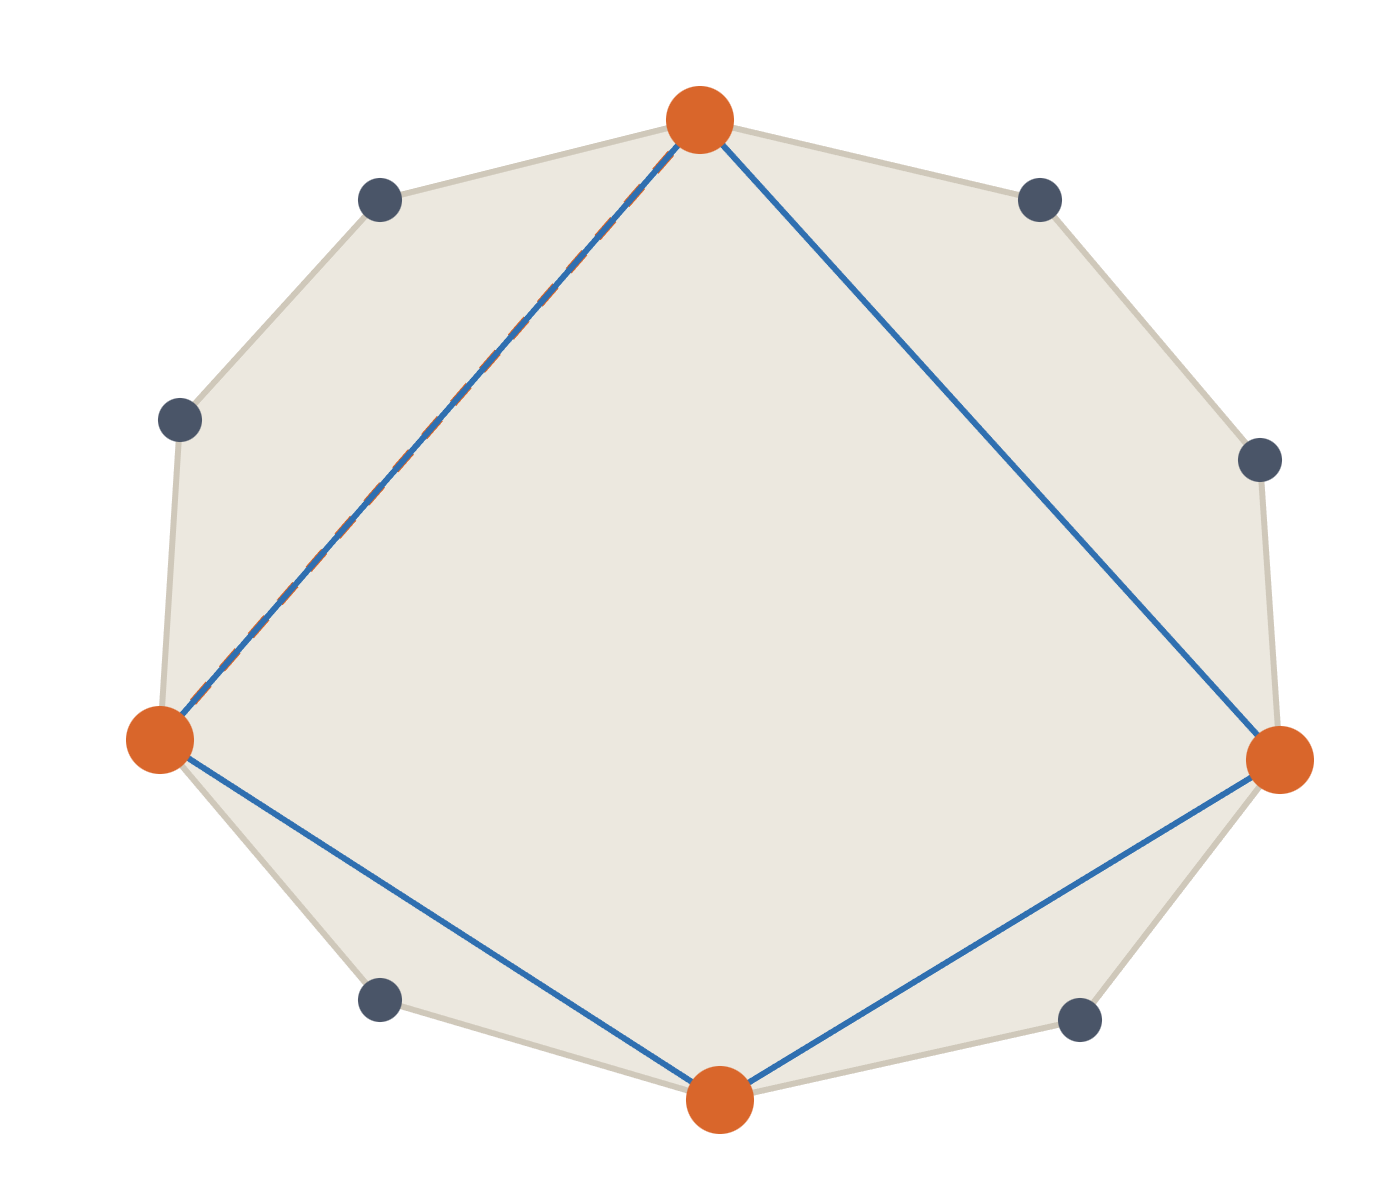
\includegraphics[width=5.4cm]{image1.png}};
\node[anchor=west,text=orng,font=\fontsize{6}{7}\selectfont\bfseries] at ([xshift=0.85cm,yshift=-1.25cm]im.north west) {closest pair};
\end{tikzpicture}
\end{column}
\end{columns}
\foot{Orange: the chosen points (k = 4). Grey: points not chosen.}
\end{frame}}

%================ 3 start
{\altslide
\begin{frame}[t]\relax
\eyebrow{WHERE WE START}
\ttl{What we add}
\vspace{10mm}
\begin{tcbraster}[raster columns=3,raster equal height,raster column skip=2.7mm]
\begin{card}\pill{Part 1}\cttl{Is the search tree correct?}\clbl{Which greedy shortcuts work, and a proof that the base paper’s search is correct for k ≤ 4.}\end{card}
\begin{card}\pill[pillb]{Part 2}\cttl{When is greedy enough?}\clbl{The arc property: one greedy walk is exact. Near-linear time for “round” point sets.}\end{card}
\begin{card}\pill{Part 3}\cttl{A simple exact algorithm}\clbl{A capped dynamic program over triangulations that always gives the exact answer.}\end{card}
\end{tcbraster}
\foot{All algorithms are implemented in C++ with exact integer arithmetic and tested against brute force.}
\end{frame}}

%================ 4
{\darkslide
\begin{frame}[c]\relax
{\head\fontsize{47}{48}\selectfont\color{lorng}01\par}\vspace{3mm}
{\head\fontsize{22.5}{24}\selectfont\color{lighttext}Greedy structure and\\the two-sided search tree\par}
\end{frame}}

%================ 5 firstfar
{\plainbg
\begin{frame}[t]\relax
\eyebrow{SECTION 4 · THE GREEDY IDEA}
\ttl{Start somewhere, take the first point far enough away}
\begin{columns}[c,onlytextwidth]
\begin{column}{0.58\textwidth}
\lead{Fix a target distance \textbf{r}. Walk around the hull from a point \textbf{q}.}\vspace{2mm}
\body{The \textbf{first far point} a(q) is the first point we meet that is at least r away from q. The pair \{q, a(q)\} is called a \textbf{tight pair}.}\vspace{2mm}
\body{Greedy: start at q, take a(q), then keep taking the next point that is far from everything chosen so far.}\vspace{2mm}
\begin{callout}Question: \hl{is there always a best solution that greedy can find?}\end{callout}
\end{column}
\begin{column}{0.36\textwidth}
\begin{tikzpicture}
\node[inner sep=0,anchor=south west] (im) at (0,0) {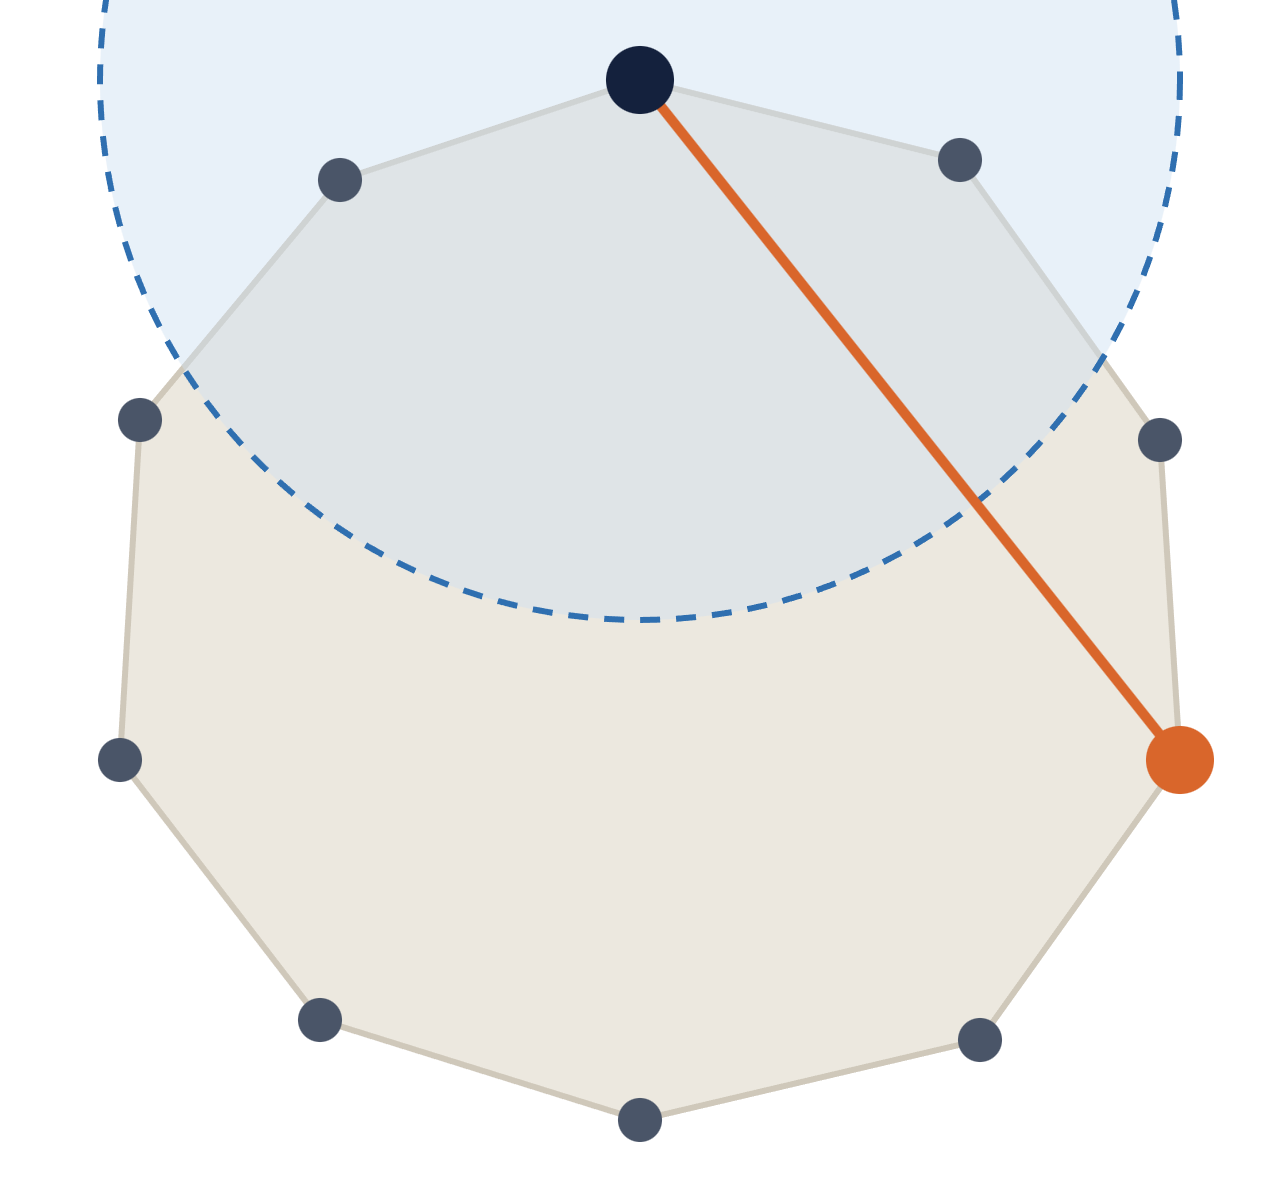
\includegraphics[width=5.33cm]{image2.png}};
\node[font=\fontsize{7}{8}\selectfont\bfseries,text=ink] at (3.15,4.82) {q};
\node[font=\fontsize{7}{8}\selectfont\bfseries,text=orng] at (4.45,1.55) {a(q)};
\node[font=\fontsize{6}{7}\selectfont,text=blu] at (1.85,2.75) {closer than r};
\end{tikzpicture}
\end{column}
\end{columns}
\end{frame}}

%================ 6 k3k4
{\altslide
\begin{frame}[t]\relax
\eyebrow{SECTION 4 · RESULT}
\ttl{Works for 3 points, breaks from 4 points on}
\begin{columns}[c,onlytextwidth]
\begin{column}{0.46\textwidth}
\begin{card}\cttl{k = 3: greedy structure holds}\clbl{Every valid triple can be turned into a “greedy” one by swapping a single point. This is why k = 3 has fast algorithms.}\end{card}
\begin{card}\cttl{k ≥ 4: it all fails}\clbl{We built 8 points where the only valid group of 4 contains no tight pair, so no greedy start can find it. Similar sets exist for k = 5, 6, 7.}\end{card}
\end{column}
\begin{column}{0.48\textwidth}
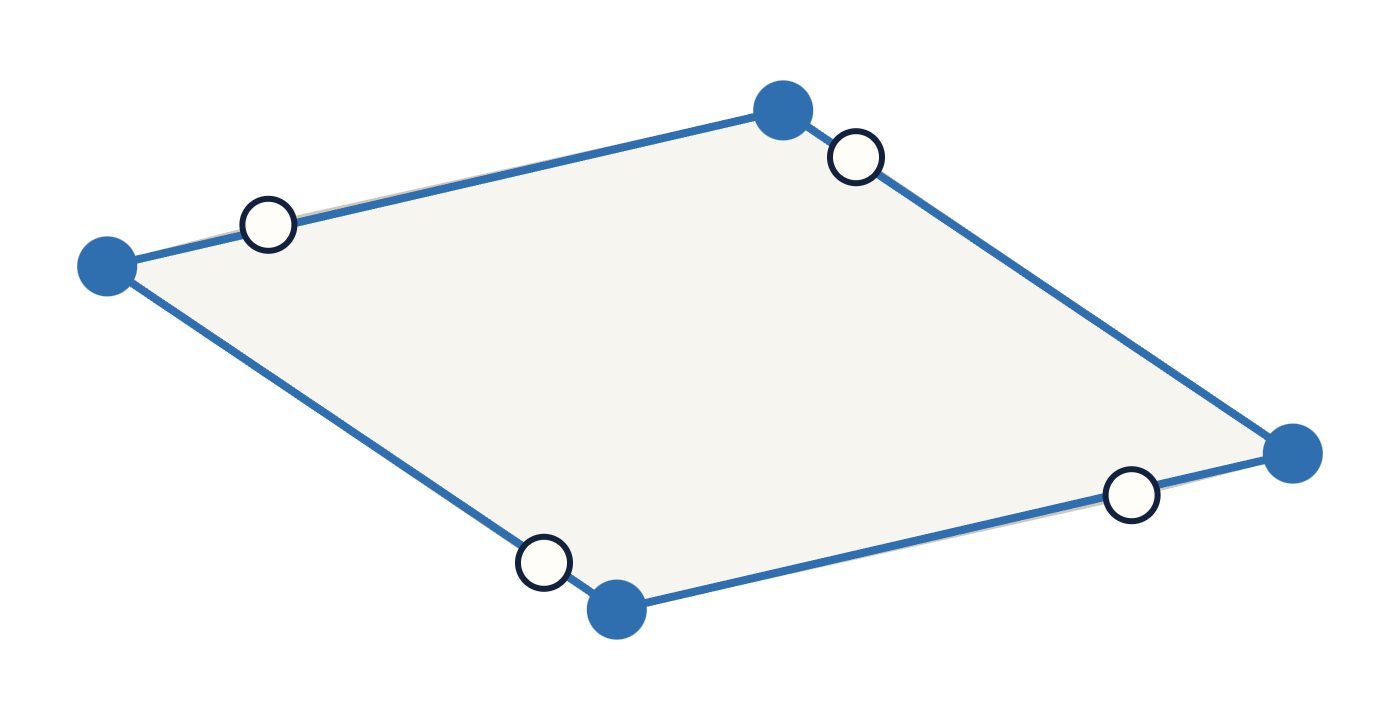
\includegraphics[width=5.8cm]{image3.png}\par\vspace{1mm}
\smalltxt{Blue: the only valid 4-set. White: each is a first far point, but too close to another blue point.}
\end{column}
\end{columns}
\end{frame}}

%================ 7 greedyres
{\plainbg
\begin{frame}[t]\relax
\eyebrow{SECTION 4 · EXPERIMENTS}
\ttl{Testing each greedy rule on millions of cases}
\begin{dtable}{@{}p{6cm}>{\raggedleft}p{2.4cm}>{\raggedleft}p{2.4cm}>{\raggedleft\arraybackslash}p{2.6cm}@{}}
\toprule
\textbf{Greedy rule} & \textbf{Cases tested} & \textbf{Failures} & \textbf{Fails for}\\\midrule
Single swap (k = 3) & 23.5 million & 0 & never\\\midrule
Arc characterisation & 173.8 million & 7.1 million & k = 4–8\\\midrule
Tight triple & 54.0 million & 107,512 & k = 4–6\\\midrule
Alternating greedy & 55.7 million & 34,474 & k = 6–12\\\midrule
Tight pair & 55.7 million & 0 random & our examples\\\bottomrule
\end{dtable}\vspace{4mm}
\begin{callout}Random testing never broke the tight-pair rule. \hl{Only hand-built and optimised examples did}, and every one is checked by brute force in exact arithmetic.\end{callout}
\end{frame}}

%================ 8 sbmtree
{\altslide
\begin{frame}[t]\relax
\eyebrow{SECTION 5 · THE BASE PAPER’S SEARCH}
\ttl{Grow the solution from one point, in both directions}
\begin{tcbraster}[raster columns=4,raster equal height,raster column skip=2.7mm]
\begin{card}\cnum{1}\cttl{Pick a start}\clbl{Choose any point q of the hull as the first chosen point.}\end{card}
\begin{card}\cnum{2}\cttl{Choose a side}\clbl{Go clockwise or anticlockwise from the chosen stretch.}\end{card}
\begin{card}\cnum{3}\cttl{Add the first far point}\clbl{Take the first point on that side that is at least r from all chosen points.}\end{card}
\begin{card}\cnum{4}\cttl{Repeat k − 1 times}\clbl{Try both sides each time: at most 2\textasciicircum k paths per start.}\end{card}
\end{tcbraster}\vspace{3mm}
\begin{callout}Fast when k is small: \hl{O(2\textasciicircum k n² log² n)}. But it is only correct if some start and some choice of sides always reaches k points. The paper’s proof of this claim is an informal picture argument.\end{callout}
\end{frame}}

%================ 9 sbmresult
{\plainbg
\begin{frame}[t]\relax
\eyebrow{SECTION 5 · WHAT WE PROVED}
\ttl{The search is correct for up to four points}
\begin{tcbraster}[raster columns=3,raster equal height,raster column skip=2.7mm]
\begin{card}\pill{Theorem}\cttl{Correct for k ≤ 4}\clbl{A full proof that the two-sided search never misses a solution of 3 or 4 points. It uses two new facts about angles in convex quadrilaterals and pentagons.}\end{card}
\begin{card}\pill[pillb]{For every k}\cttl{The first step is always safe}\clbl{Using the “ears” of a Delaunay triangulation, we show the search can always make its first move without losing the solution.}\end{card}
\begin{card}\pill{Counterexamples}\cttl{Simple start rules fail}\clbl{Starting at a closest pair fails for k = 5, 6. Starting at the sharpest corner fails for k = 7.}\end{card}
\end{tcbraster}\vspace{3mm}
\begin{callout}The base paper’s algorithm is now \hl{proven correct for k ≤ 4}, and we know the start point must be chosen with care.\end{callout}
\end{frame}}

%================ 10 sbmres
{\altslide
\begin{frame}[t]\relax
\eyebrow{SECTION 5 · IMPLEMENTATION AND EXPERIMENTS}
\ttl{Checking the search tree in code}
\begin{tcbraster}[raster columns=3,raster equal height,raster column skip=2.7mm]
\begin{card}\cnum{29 M}\clbl{random cases with k = 4 checked against the proof: no failure}\end{card}
\begin{card}\cnum[blu]{532,833}\clbl{random tests plus about 3,000 adversarial runs for k ≤ 10: the search always succeeded}\end{card}
\begin{card}\cnum{10–14}\clbl{points in our counterexamples to the start rules, verified by exhaustive search}\end{card}
\end{tcbraster}\vspace{2mm}
{\fontsize{7.6}{11}\selectfont\color{soft}
\begin{itemize}\setlength{\itemsep}{1mm}
\item We re-implemented the base paper’s search tree and dynamic program in C++ (folder \textbf{sbm/}).
\item Adversarial runs move points on purpose to make the search fail; this is how the start-rule counterexamples were found.
\item All distances are compared as exact integers, so no answer depends on rounding.
\end{itemize}}
\end{frame}}

%================ 11
{\darkslide
\begin{frame}[c]\relax
{\head\fontsize{47}{48}\selectfont\color{lorng}02\par}\vspace{3mm}
{\head\fontsize{22.5}{24}\selectfont\color{lighttext}When greedy is exact:\\the arc property\par}
\end{frame}}

%================ 12 arcidea
{\plainbg
\begin{frame}[t]\relax
\eyebrow{SECTION 6 · THE ARC PROPERTY}
\ttl{The far points of every point form one stretch}
\begin{columns}[t,onlytextwidth]
\begin{column}{0.48\textwidth}\centering
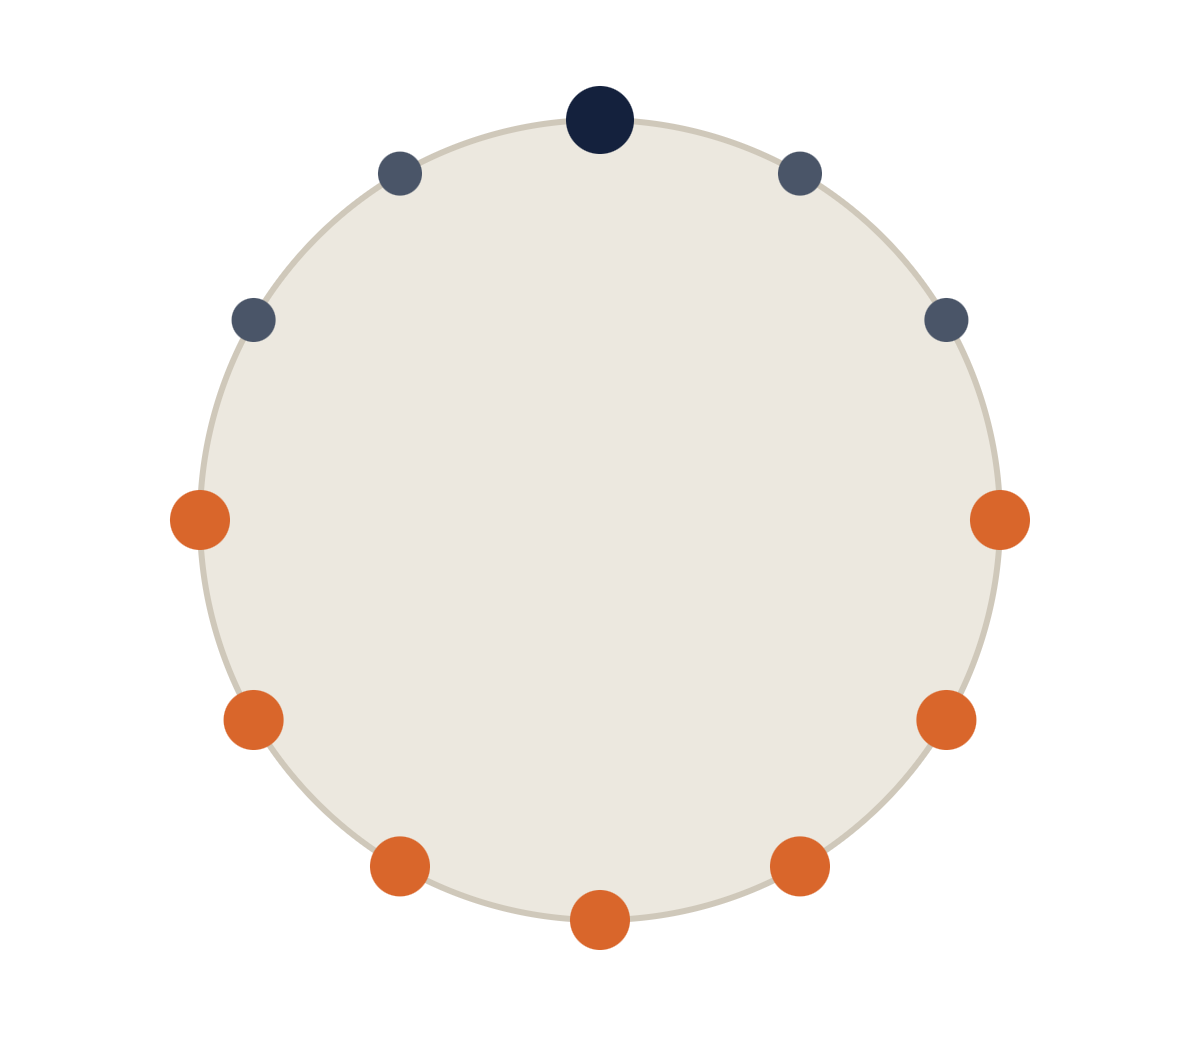
\includegraphics[width=4.6cm]{image4.png}\par\vspace{1mm}
\pill{Round shape: one stretch — property holds}
\end{column}
\begin{column}{0.48\textwidth}\centering
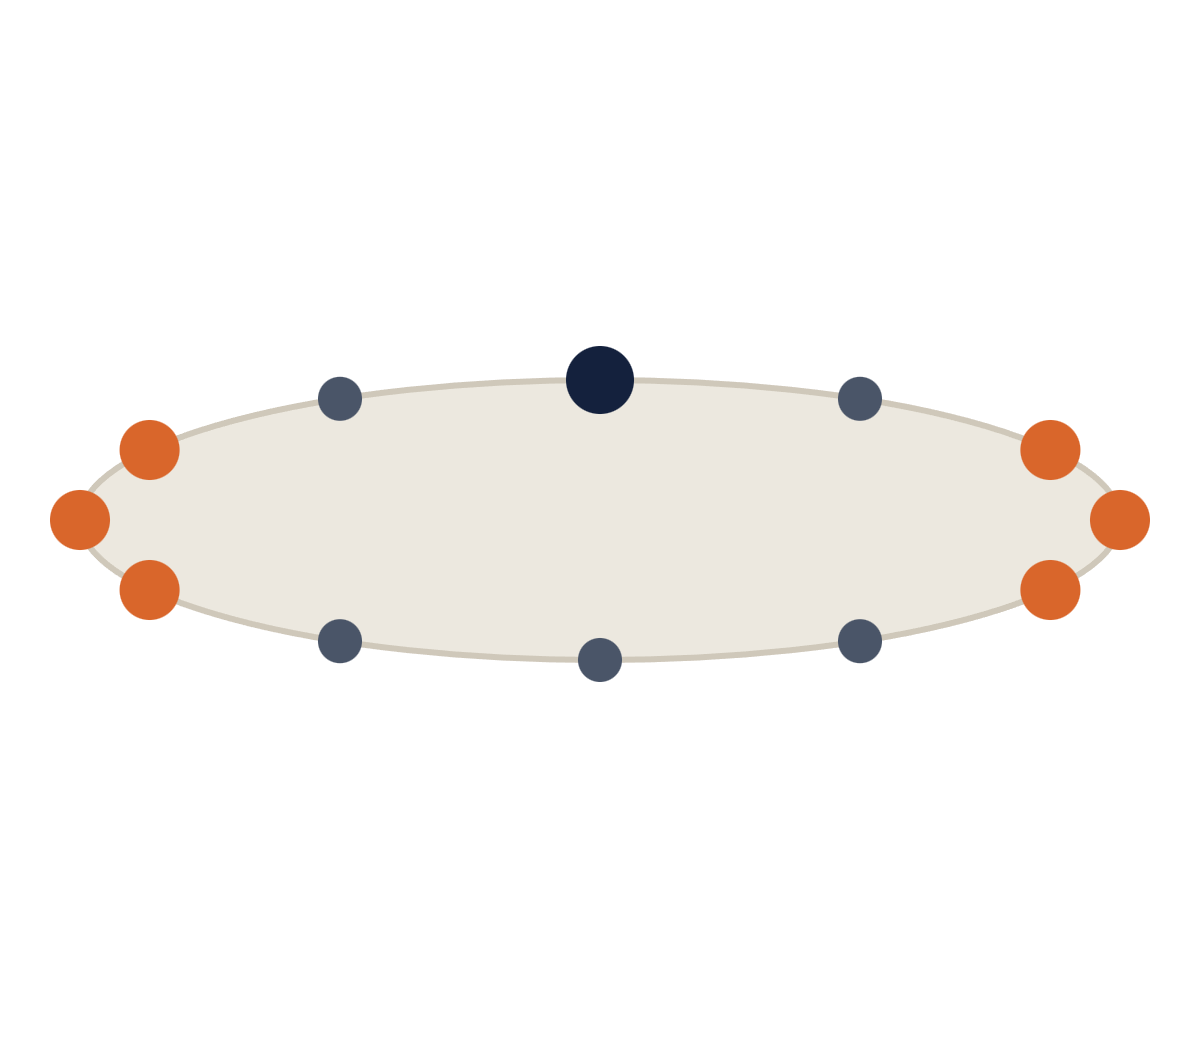
\includegraphics[width=4.6cm]{image5.png}\par\vspace{1mm}
\pill[pillb]{Thin shape: two pieces — property fails}
\end{column}
\end{columns}
\foot{Dark point: q. Orange: points at least r away from q. Grey: points closer than r.}
\end{frame}}

%================ 13 chain
{\altslide
\begin{frame}[t]\relax
\eyebrow{SECTION 6 · MAIN THEOREM}
\ttl{With the arc property, one greedy walk is enough}
\begin{columns}[c,onlytextwidth]
\begin{column}{0.58\textwidth}
\lead{Start anywhere. Keep jumping to the \textbf{first far point}. Stop when the walk comes back around.}\vspace{2mm}
\body{If the walk fits k jumps before it returns to the start, the answer is \textbf{yes}; if not, it is \textbf{no}. No branching, no backtracking.}\vspace{2mm}
\begin{callout}Decision in \hl{O(n log n)} time, and the base paper’s claim holds with no branching at all.\end{callout}
\end{column}
\begin{column}{0.37\textwidth}
\begin{tikzpicture}
\node[inner sep=0,anchor=south west] at (0,0) {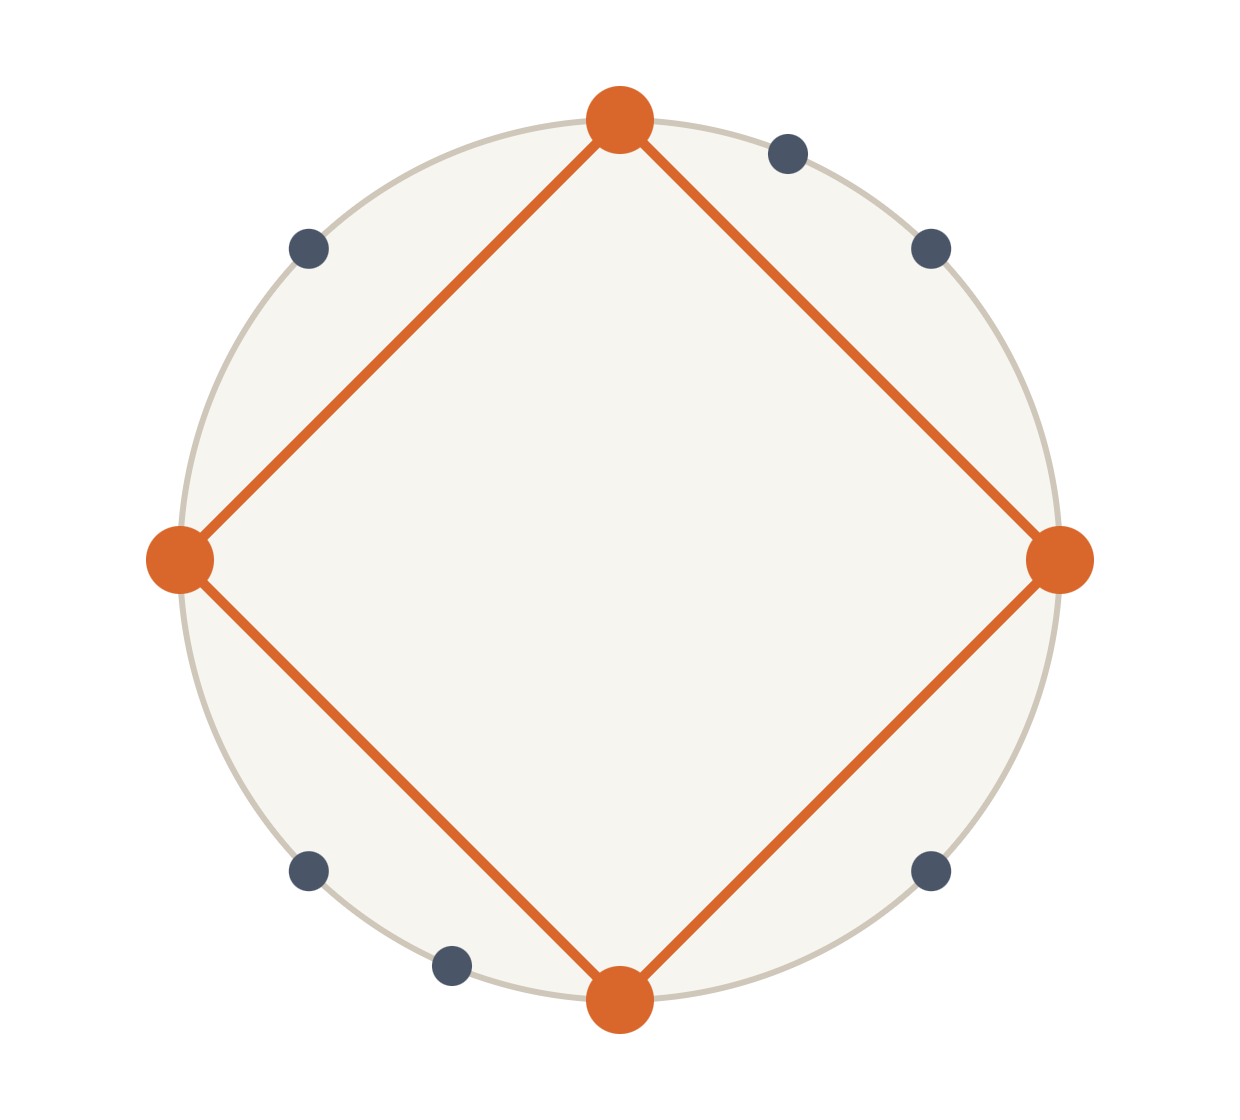
\includegraphics[width=5.17cm]{image6.png}};
\foreach \x/\y/\t/\c in {3.0/4.55/start/ink, 4.0/3.0/1/orng, 2.95/0.35/2/orng, 0.45/3.0/3/orng}
  \node[font=\fontsize{7}{8}\selectfont\bfseries,text=\c] at (\x,\y) {\t};
\end{tikzpicture}
\end{column}
\end{columns}
\end{frame}}

%================ 14 unimodal
{\plainbg
\begin{frame}[t]\relax
\eyebrow{SECTION 6 · UNIMODAL POINT SETS}
\ttl{Round shapes get a near-linear algorithm}
\begin{tcbraster}[raster columns=3,raster equal height,raster column skip=2.7mm]
\begin{card}\pill{What it means}\cttl{Unimodal set}\clbl{From every point, distances around the hull go up and then down. Points on a circle, or slightly moved from one, are unimodal.}\end{card}
\begin{card}\pill[pillb]{Why it helps}\cttl{Arc property at every r}\clbl{So the greedy walk is exact for every distance we try, and we can search for the best distance quickly.}\end{card}
\begin{card}\pill{Safety check}\cttl{Test it first}\clbl{Whether a set is unimodal can be checked exactly in O(n log n) time before we run.}\end{card}
\end{tcbraster}\vspace{3mm}
\begin{callout}Exact answer in expected \hl{O(n log² n)} time, compared with about n³ for general point sets.\end{callout}
\end{frame}}

%================ 15 arcres
{\altslide
\begin{frame}[t]\relax
\eyebrow{SECTION 6 · IMPLEMENTATION AND EXPERIMENTS}
\ttl{Exact on every test, and fast at a million points}
\begin{columns}[t,onlytextwidth]
\begin{column}{0.52\textwidth}
\begin{dtable}{@{}p{2.5cm}>{\raggedleft}p{2.2cm}>{\raggedleft\arraybackslash}p{2.4cm}@{}}
\toprule
\textbf{Points n} & \textbf{Cubic DP} & \textbf{Our algorithm}\\\midrule
400 & 4.7 s & 0.4 ms\\\midrule
10,000 & not run & 19 ms\\\midrule
100,000 & not run & 0.56 s\\\midrule
1,000,000 & not run & 8.2 s\\\bottomrule
\end{dtable}\par\vspace{1.5mm}
\smalltxt{k = 16, median of three unimodal instances; 128-bit arithmetic from 100,000 points.}
\end{column}
\begin{column}{0.42\textwidth}
\begin{card}\cnum{2.65 M}\clbl{answers compared with brute force: no mismatch}\end{card}
\begin{card}\cnum[blu]{≈ n\textasciicircum1.15}\clbl{measured growth, close to linear}\end{card}
\end{column}
\end{columns}\vspace{2mm}
\smalltxt{On thin shapes the property fails, and running the walk without checking gave wrong answers in 8\% of cases. That is why the algorithm tests the property first.}
\end{frame}}

%================ 16
{\darkslide
\begin{frame}[c]\relax
{\head\fontsize{47}{48}\selectfont\color{lorng}03\par}\vspace{3mm}
{\head\fontsize{22.5}{24}\selectfont\color{lighttext}A simple exact algorithm:\\the capped dynamic program\par}
\end{frame}}

%================ 17 certificate
{\plainbg
\begin{frame}[t]\relax
\ttl{Checking “all pairs far apart” using only triangles}
\begin{columns}[c,onlytextwidth]
\begin{column}{0.58\textwidth}
\lead{A set of k points is valid exactly when it can be cut into triangles whose \textbf{edges are all at least r long} and whose diagonals are \textbf{Delaunay} (no fourth point inside a triangle’s circle).}\vspace{2mm}
\body{So we never compare every pair. We only build triangles, one diagonal at a time, and test small local conditions.}\vspace{2mm}
\begin{callout}This turns a global condition into \hl{local checks}, which is exactly what a dynamic program needs.\end{callout}
\end{column}
\begin{column}{0.37\textwidth}
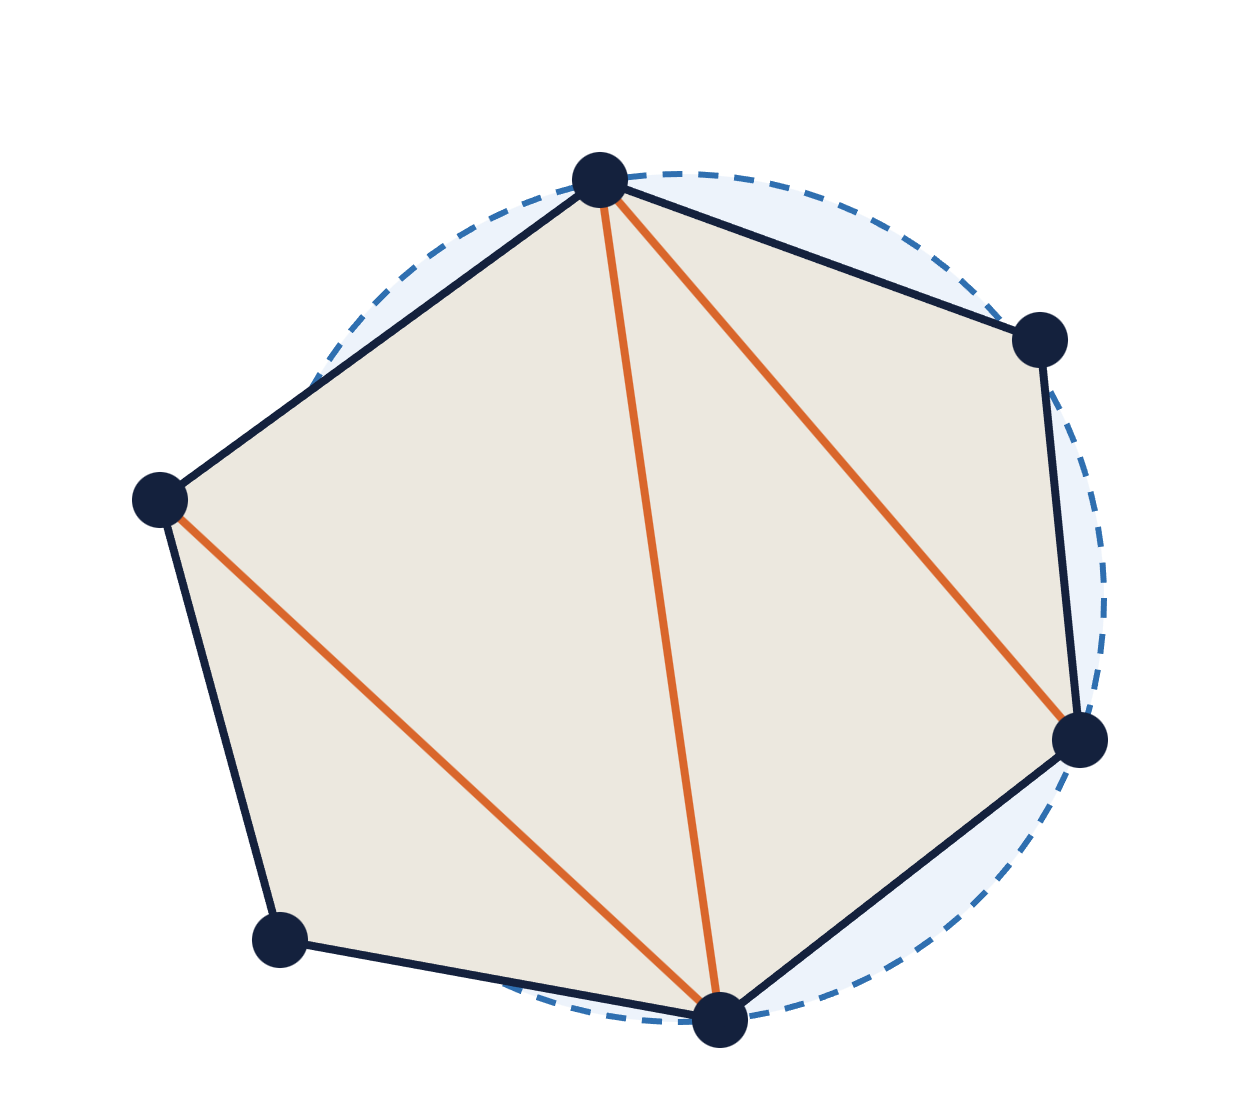
\includegraphics[width=5.17cm]{image7.png}
\end{column}
\end{columns}
\foot{Orange: diagonals of the triangulation. Dashed: the circle through one triangle, with no other chosen point inside.}
\end{frame}}

%================ 18 capdp
{\altslide
\begin{frame}[t]\relax
\eyebrow{SECTION 7 · THE ALGORITHM}
\ttl{A dynamic program over chords, with a cap}
\begin{tcbraster}[raster columns=3,raster equal height,raster column skip=2.7mm]
\begin{card}\cnum{1}\cttl{Work chord by chord}\clbl{For every chord of the polygon, from short to long, ask: how many far-apart points fit on one side of it?}\end{card}
\begin{card}\cnum{2}\cttl{Glue triangles}\clbl{A bigger answer comes from two smaller chords plus one triangle that passes the local Delaunay check.}\end{card}
\begin{card}\cnum{3}\cttl{Cap at k − 2}\clbl{We never need more than k − 2 numbers per chord, so we stop there. Most of the work disappears.}\end{card}
\end{tcbraster}\vspace{3mm}
\begin{dtable}{@{}p{7.2cm}>{\raggedleft\arraybackslash}p{6.6cm}@{}}
\toprule
\textbf{Exact algorithm (decision: “is r reachable?”)} & \textbf{Time}\\\midrule
Base paper’s dynamic program & O(n⁴ k²)\\\midrule
Tkachenko and Wang (SWAT 2026) & O(n³ log n)\\\midrule
Our capped dynamic program & O(n³ log k)\\\bottomrule
\end{dtable}
\end{frame}}

%================ 19 window
{\plainbg
\begin{frame}[t]\relax
\eyebrow{SECTION 7 · FINDING THE BEST DISTANCE}
\ttl{Search only where the answer can be}
\begin{columns}[t,onlytextwidth]
\begin{column}{0.47\textwidth}
{\head\fontsize{9.5}{12}\selectfont\color{ink}Search window\par}\vspace{1.5mm}
\body{A quick greedy (always take the point farthest from those chosen) gives a distance \textbf{g}. The true answer is guaranteed to lie between \textbf{g} and \textbf{2g}, and below perimeter ÷ k.}\vspace{1.5mm}
\body{So binary search only looks at distances in that window.}
\end{column}
\begin{column}{0.47\textwidth}
{\head\fontsize{9.5}{12}\selectfont\color{ink}Certified algorithm\par}\vspace{1.5mm}
\body{Greedy rules are fast and never give a wrong set, but may give a smaller distance than the best.}\vspace{1.5mm}
\body{So we run greedy first, then \textbf{one exact check} just above its answer. If that check says “no”, greedy was optimal and we are done.}
\end{column}
\end{columns}\vspace{4mm}
\begin{callout}Full optimisation in \hl{O(n³ log k log n)} time, and usually only one or two exact checks in practice.\end{callout}
\end{frame}}

%================ 20 dpres
{\altslide
\begin{frame}[t]\relax
\eyebrow{SECTION 7 · IMPLEMENTATION AND EXPERIMENTS}
\ttl{Always exact, and the speed-ups pay off}
\begin{tcbraster}[raster columns=3,raster equal height,raster column skip=2.7mm]
\begin{card}\cnum{846 / 846}\clbl{instances solved correctly, checked against brute force and independent code}\end{card}
\begin{card}\cnum[blu]{6\%}\clbl{of all distances fall in the search window (median)}\end{card}
\begin{card}\cnum{95\%}\clbl{of instances: greedy was already optimal and one exact check confirmed it}\end{card}
\end{tcbraster}\vspace{3mm}
\begin{dtable}{@{}p{4.3cm}>{\raggedleft}p{3cm}>{\raggedleft}p{3cm}>{\raggedleft\arraybackslash}p{3cm}@{}}
\toprule
\textbf{k (n = 200)} & \textbf{Without cap} & \textbf{With cap} & \textbf{Certified}\\\midrule
4 & 41 ms & 23 ms & 7 ms\\\midrule
16 & 1.06 s & 0.77 s & 0.10 s\\\midrule
64 & 2.45 s & 2.15 s & 0.28 s\\\bottomrule
\end{dtable}
\end{frame}}

%================ 21 summary
{\plainbg
\begin{frame}[t]\relax
\eyebrow{SUMMARY}
\ttl{What the project adds}
\begin{dtable}{@{}p{5.9cm}p{3.6cm}p{4.3cm}@{}}
\toprule
\textbf{Result} & \textbf{Before} & \textbf{Now}\\\midrule
Base paper’s search tree & informal proof & proven correct for k ≤ 4\\\midrule
Greedy rules for k ≥ 4 & unknown & all fail, with small examples\\\midrule
Round (unimodal) point sets & about n³ time & O(n log² n) expected\\\midrule
Exact decision, any convex set & O(n³ log n) & O(n³ log k)\\\midrule
Implementation & — & C++, exact arithmetic, all tests pass\\\bottomrule
\end{dtable}\vspace{4mm}
\begin{callout}Proofs where there were pictures, a \hl{near-linear algorithm} for round inputs, and a \hl{simpler exact algorithm} for all inputs.\end{callout}
\end{frame}}

%================ 22 thanks
{\darkslide
\begin{frame}[c]\relax
{\head\fontsize{22.5}{24}\selectfont\color{lighttext}Thank you\par}\vspace{3mm}
{\fontsize{9.5}{12}\selectfont\color{darktext}Questions?\par}\vspace{8mm}
{\fontsize{7}{10}\selectfont\color{darktext}Akshat Bharara · Rakshith Ashok Kumar · Utsav Singh Bhamra\\Guide: Prof. Manjanna B · NITK Surathkal\par}
\end{frame}}

\end{document}
